%!Tex Root=**/main.tex

\section{MonoGS}

\subsection{Methodology}

\begin{Frame}{Overview \romannum{1}}
	\begin{figure}[htbp]
		\centering
		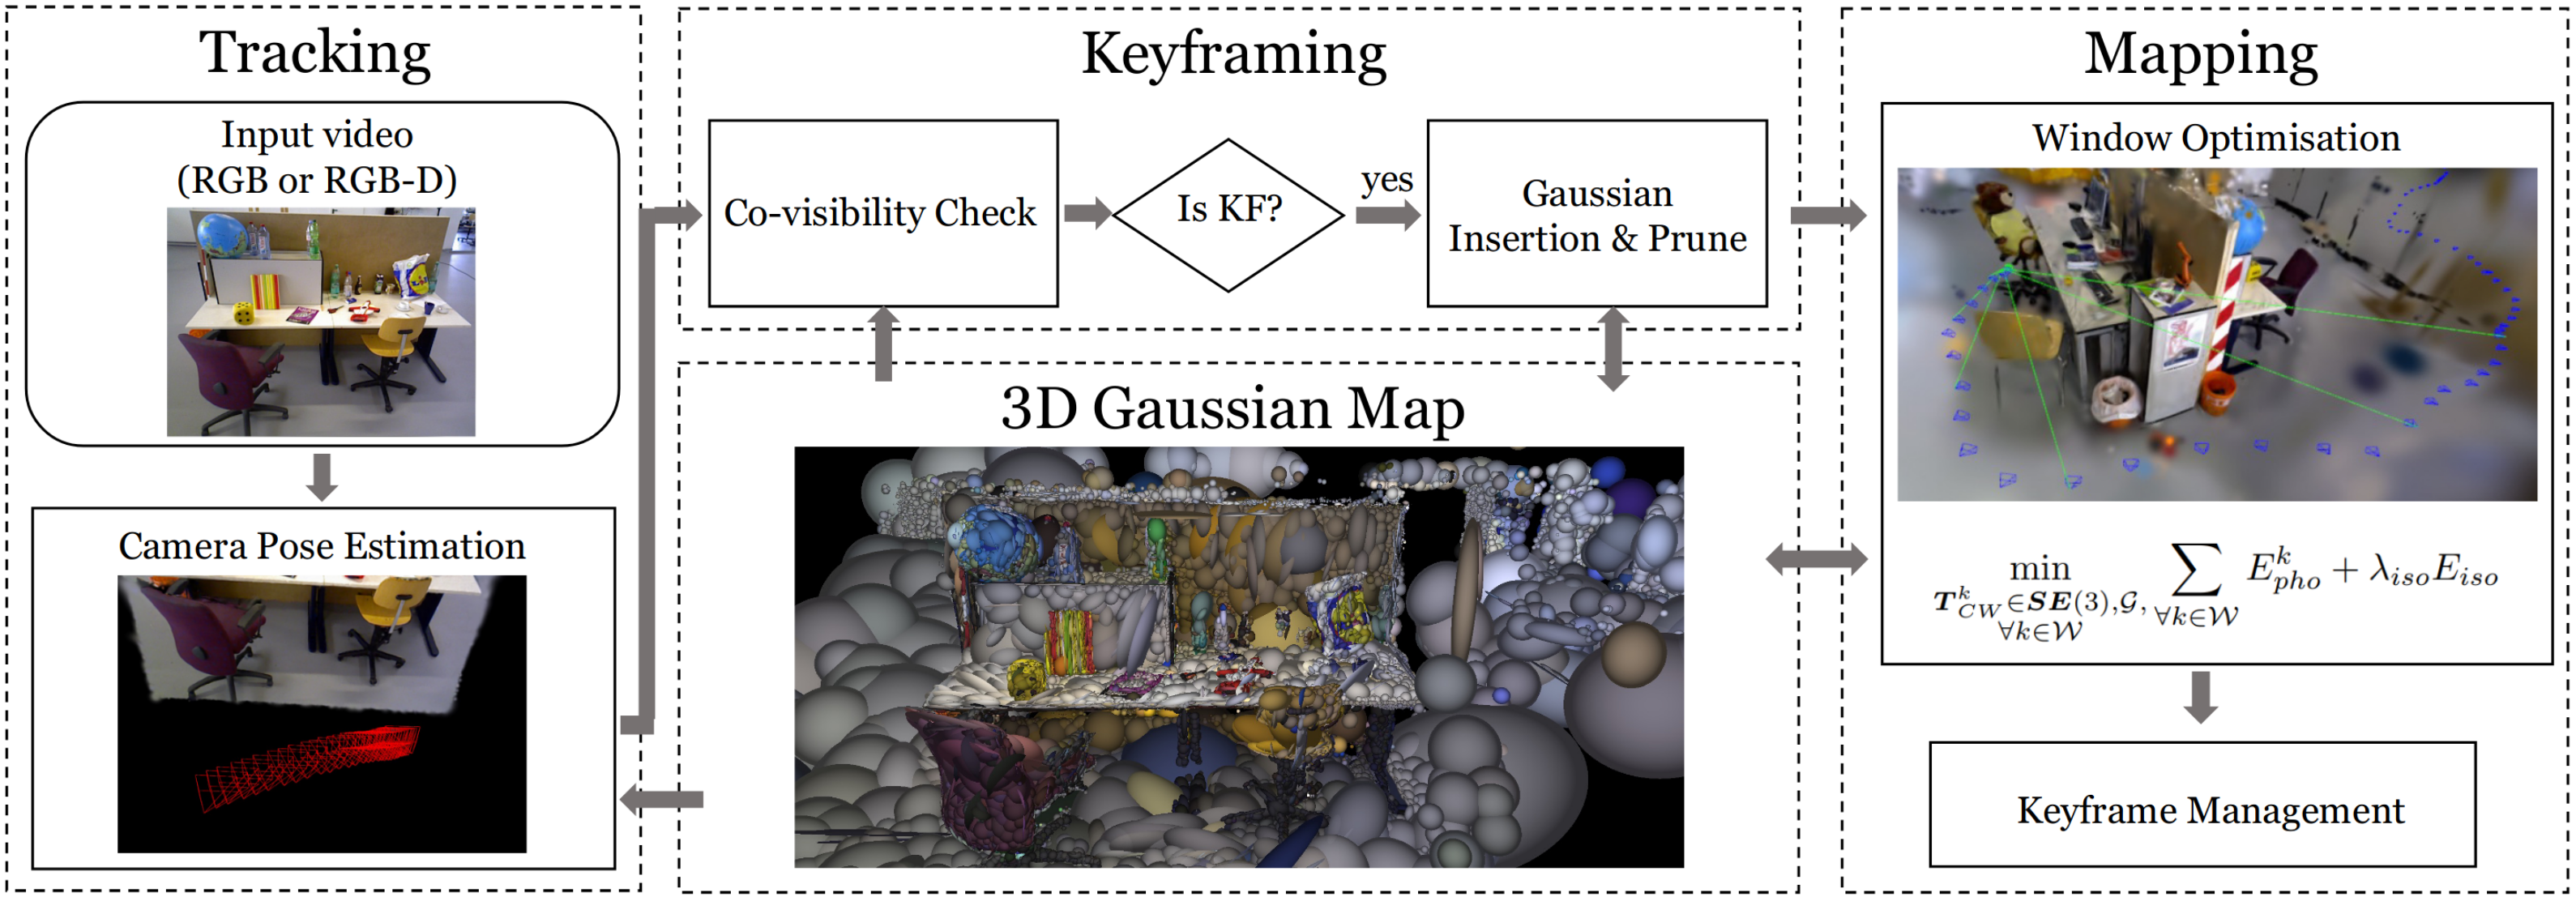
\includegraphics[width=\linewidth]{monogs/overview.png}
	\end{figure}
	\blfootnote{\href{http://arxiv.org/abs/2312.06741}{(CVPR Highlight, 2024) MonoGS: Gaussian Splatting SLAM}}
\end{Frame}

\tikzset{
	key/.style={
			draw=OrangeRed,
		},
	convention/.style={
			draw=Cerulean,
		},
	trick/.style={
			draw=ForestGreen,
		},
}
\begin{Frame}{Overview \romannum{2}}
	\centering
	\resizebox{0.85\textwidth}{!}{
		\begin{forest}
			for tree={my tree}
			[
			MonoGS
				[
					Visual Odometry,for children={visible on=<1->}
						[
							Tracking,for children={visible on=<2->}
								[
									``Inverse Rendering'',for children={visible on=<3->}
										[
											Analytical Jacobians Derivation,key
										]
										[
											Photometric RGB \& Depth Loss,convention
										]
										[
											Optimizable Exposure,trick
										]
										[
											Penalization on non-edge/low-opacity pixels,trick
										]
								]
						]
						[
							Mapping,for children={visible on=<2->}
								[
									Bundle Adjustment,for children={visible on=<3->}
										[
											Photometric RGB \& Depth Loss,convention
										]
										[
											Isotropic Regularization,key
										]
										[
											Random Recall,trick
										]
								]
						]
				]
				[
					Online Pipeline,for children={visible on=<1->}
						[
							Keyframe Management,for children={visible on=<2->}
								[
									Registration,for children={visible on=<3->}
										[
											Gaussian Covisibility,key
										]
										[
											Relative Translation,convention
										]
								]
								[
									Removal,for children={visible on=<3->}
										[
											Gaussian Overlap Coefficient,key
										]
								]
						]
						[
							Gaussian Management,for children={visible on=<2->}
								[
									Insertion,for children={visible on=<3->}
										[
											Keyframing,convention
										]
								]
								[
									Pruning,for children={visible on=<3->}
										[
											Gaussian Covisibility,key
										]
								]
						]
				]
			]
		\end{forest}
	}
	\resizebox{0.08\textwidth}{!}{
		\begin{tikzpicture}[visible on=<3->]
			\node [my node for tree, draw=ForestGreen] (trick node) {trick};
			\node [my node for tree, draw=OrangeRed, above of = trick node] {key method};
			\node [my node for tree, draw=Cerulean, below of = trick node] (convention) {convention};
		\end{tikzpicture}
	}
	\blfootnote{\href{http://arxiv.org/abs/2312.06741}{(CVPR Highlight, 2024) MonoGS: Gaussian Splatting SLAM}}
\end{Frame}

\begin{Frame}{Tracking: Overview}
	\begin{figure}[htbp]
		\centering
		\resizebox{0.7\textwidth}{!}{
			\begin{forest} for tree={my tree}
				[
				Tracking
				[
				``Inverse Rendering''
				[
				Analytical Jacobians Derivation,key
				]
				[
				Photometric RGB \& Depth Loss,convention
				]
				[
				Optimizable Exposure,trick
				]
				[
				Penalization on non-edge/low-opacity pixels,trick
				]
				]
				]
			\end{forest}
		}
	\end{figure}
	\vspace*{\fill}
	\par Track camera poses,
	\vspace*{1.5ex}
	\begin{itemize}[<+->]
		\setlength{\itemsep}{1.5ex}
		\item \textcolor{OrangeRed}{through the extended differentiable rendering pipeline},
		\item \textcolor{Cerulean}{by a direct optimization against fixed 3D Gaussians,}
		\item \textcolor{ForestGreen}{with some tricks to be more adaptive to brightness and more robust to noise.}
	\end{itemize}
	\blfootnote{
		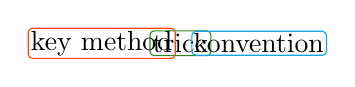
\begin{tikzpicture}
			\node [inner sep=1pt, rounded corners=1.5, draw=ForestGreen] (trick node) {trick};
			\node [inner sep=1pt, rounded corners=1.5, draw=OrangeRed, left of = trick node] {key method};
			\node [inner sep=1pt, rounded corners=1.5, draw=Cerulean, right of = trick node] (convention) {convention};
		\end{tikzpicture}
	}
	\blfootnote{\href{http://arxiv.org/abs/2312.06741}{(CVPR Highlight, 2024) MonoGS: Gaussian Splatting SLAM}}
\end{Frame}

\begin{Frame}{Tracking: A Review of 3DGS}
	\vspace*{-5em}
	\par The projection from ``ellipsoids'' to ``ellipses'' in 3DGS,
	\begin{equation}
		\mathcal{N}\left(\mu_w, \Sigma_w\right) \overset{\pi}{\mapsto} \mathcal{N}\left(\mu_i, \Sigma_i\right),
	\end{equation}
	is achieved by,
	\begin{overprint}[0.8\textheight]
		\usetikzlibrary{overlay-beamer-styles}
		\begin{figure}[htbp]
			\centering
			\begin{minipage}[c]{0.35\linewidth}
				\begin{onlyenv}<1>
					\begin{equation}
						\mu_{i} = \pi \left( \mathbf{T}_{cw} \cdot \mu_{w} \right)
					\end{equation}
				\end{onlyenv}
				\begin{onlyenv}<2->
					\begin{equation*}
						\resetcolorseries[4]{marknode-color-series}
						\tikzmarknode{n0}{\colorbox{marknode-color-series!![0]}{\(\mu_{i}\)}} = \tikzmarknode{n1}{\colorbox{marknode-color-series!![1]}{\(\pi\)}} \left( \tikzmarknode{n2}{\colorbox{marknode-color-series!![2]}{\(\mathbf{T}_{cw}\)}} \cdot \tikzmarknode{n3}{\colorbox{marknode-color-series!![3]}{\(\mu_{w}\)}} \right)
					\end{equation*}
					\begin{annotatedEquationEnv}
						\resetcolorseries[4]{annotation-color-series}
						\annotatedEquation{colorseries}{n0}{south}{0}{-7em}{north west}{annotation-color-series}{\(\in \mathbb{P}^2\), 2D(image) mean}{east}
						\annotatedEquation{colorseries}{n1}{south}{0em}{-5em}{north west}{annotation-color-series}{projection}{east}
						\annotatedEquation{colorseries}{n2}{south}{0em}{-3em}{north west}{annotation-color-series}{\(\in \mathrm{SE}(3)\), camera pose}{east}
						\annotatedEquation{colorseries}{n3}{south}{0em}{-1em}{north west}{annotation-color-series}{\(\in \mathbb{P}^3\), 3D(world) mean}{east}
					\end{annotatedEquationEnv}
				\end{onlyenv}
			\end{minipage}
			\begin{minipage}[c]{0.60\linewidth}
				\begin{onlyenv}<1>
					\begin{equation}
						\Sigma_{i} = \mathbf{J}_{\pi} \mathbf{R}_{cw} \Sigma_{w} \mathbf{R}_{cw}^{\mathrm{T}} \mathbf{J}_{\pi}^{\mathrm{T}}
					\end{equation}
				\end{onlyenv}
				\begin{onlyenv}<2->
					\begin{equation*}
						\resetcolorseries[4]{marknode-color-series}
						\tikzmarknode{n4}{\colorbox{marknode-color-series!![4]}{\(\Sigma_{i}\)}} = \tikzmarknode{n5}{\colorbox{marknode-color-series!![5]}{\(\mathbf{J}_{\pi}\)}} \tikzmarknode{n6}{\colorbox{marknode-color-series!![6]}{\(\mathbf{R}_{cw}\)}} \tikzmarknode{n7}{\colorbox{marknode-color-series!![7]}{\(\Sigma_{w}\)}} \mathbf{R}_{cw}^{\mathrm{T}} \mathbf{J}_{\pi}^{\mathrm{T}}
					\end{equation*}
					\begin{annotatedEquationEnv}
						\resetcolorseries[4]{annotation-color-series}
						\annotatedEquation{colorseries}{n4}{south}{0em}{-7em}{north west}{annotation-color-series}{\(\in \mathbb{R}^{2\times 2}\), 2D(image) covariance}{east}
						\annotatedEquation{colorseries}{n5}{south}{0em}{-5em}{north west}{annotation-color-series}{\(\in \mathbb{R}^{2\times 3}\), Jacobian of the linear approximation of \(\pi\)}{east}
						\annotatedEquation{colorseries}{n6}{south}{0em}{-3em}{north west}{annotation-color-series}{\(\in \mathrm{SO(3)}\), rotation component of \(\mathbf{T}_{cw}\)}{east}
						\annotatedEquation{colorseries}{n7}{south}{0em}{-1em}{north west}{annotation-color-series}{\(\in \mathbb{R}^{3\times 3}\), 3D(world) covariance}{east}
					\end{annotatedEquationEnv}
				\end{onlyenv}
			\end{minipage}
		\end{figure}
	\end{overprint}
	\blfootnote{\href{http://arxiv.org/abs/2312.06741}{(CVPR Highlight, 2024) MonoGS: Gaussian Splatting SLAM}}
\end{Frame}

\begin{Frame}{Tracking: Derivation of Jacobians \romannum{1}}
	\par The chain rule,
	\begin{alignat}{1}
		\frac{\partial \mu_i}{\partial \mathbf{T}_{cw}}    & = \frac{\partial \mu_i}{\partial \mu_c} \frac{\partial \mu_c}{\partial \mathbf{T}_{cw}}                                                                                                                                                                               \\
		\frac{\partial \Sigma_i}{\partial \mathbf{T}_{cw}} & = \frac{\partial \Sigma_i}{\partial \mathbf{J}_{\pi}} \frac{\partial \mathbf{J}_{\pi}}{\partial \mu_c} \frac{\partial \mu_c}{\partial \mathbf{T}_{cw}} + \frac{\partial \Sigma_i}{\partial \mathbf{R}_{cw}} \frac{\partial \mathbf{R}_{cw}}{\partial \mathbf{T}_{cw}}
	\end{alignat}
	\pause
	\par The Lie Algebra,
	\begin{alignat}{1}
		\frac{\partial \mu_c}{\partial \mathbf{T}_{cw}}           & = \begin{bmatrix}
			                                                              \mathbf{I} & -\mu_{c}^{\times}
		                                                              \end{bmatrix}               \\
		\frac{\partial \mathbf{R}_{cw}}{\partial \mathbf{T}_{cw}} & = \begin{bmatrix}
			                                                              \mathbf{0} & - \mathbf{R}_{cw}^{\times}(:,1) \\
			                                                              \mathbf{0} & - \mathbf{R}_{cw}^{\times}(:,2) \\
			                                                              \mathbf{0} & - \mathbf{R}_{cw}^{\times}(:,3) \\
		                                                              \end{bmatrix}
	\end{alignat}
	\blfootnote{\href{http://arxiv.org/abs/2312.06741}{(CVPR Highlight, 2024) MonoGS: Gaussian Splatting SLAM}}
\end{Frame}

\begin{Frame}{Online Pipeline: Overview}
	\begin{figure}[htbp]
		\centering
		\resizebox{0.8\textwidth}{!}{
			\begin{forest}
				for tree={my tree}
				[
				Online Pipeline
					[
						Keyframe Management
							[
								Registration
									[
										Gaussian Covisibility,key
									]
									[
										Relative Translation,convention
									]
							]
							[
								Removal
									[
										Gaussian Overlap Coefficient,key
									]
							]
					]
					[
						Gaussian Management
							[
								Insertion
									[
										Keyframing,convention
									]
							]
							[
								Pruning
									[
										Gaussian Covisibility,key
									]
							]
					]
				]
			\end{forest}
		}
	\end{figure}
	\par Keyframe Management:
	\vspace*{1.5ex}
	\begin{itemize}[<+-| alert@+>]
		\setlength{\itemsep}{1.5ex}
		\item Classic keyframing strategies from DSO~\autocite{engel2016dso}.
		\item Occlusion-aware Gaussian visibility is leveraged to construct covisibility and overlap metrics.
	\end{itemize}
	\blfootnote{
		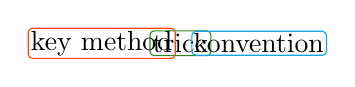
\begin{tikzpicture}
			\node [inner sep=1pt, rounded corners=1.5, draw=ForestGreen] (trick node) {trick};
			\node [inner sep=1pt, rounded corners=1.5, draw=OrangeRed, left of = trick node] {key method};
			\node [inner sep=1pt, rounded corners=1.5, draw=Cerulean, right of = trick node] (convention) {convention};
		\end{tikzpicture}
	}
	\blfootnote{\href{http://arxiv.org/abs/1607.02565}{(arXiv, 2016) DSO: Direct Sparse Odometry}}
	\blfootnote{\href{http://arxiv.org/abs/2312.06741}{(CVPR Highlight, 2024) MonoGS: Gaussian Splatting SLAM}}
\end{Frame}

\begin{Frame}{Online Pipeline: Overview}
	\begin{figure}[htbp]
		\centering
		\resizebox{0.8\textwidth}{!}{
			\begin{forest}
				for tree={my tree}
				[
				Online Pipeline
					[
						Keyframe Management
							[
								Registration
									[
										Gaussian Covisibility,key
									]
									[
										Relative Translation,convention
									]
							]
							[
								Removal
									[
										Gaussian Overlap Coefficient,key
									]
							]
					]
					[
						Gaussian Management
							[
								Insertion
									[
										Keyframing,convention
									]
							]
							[
								Pruning
									[
										Gaussian Covisibility,key
									]
							]
					]
				]
			\end{forest}
		}
	\end{figure}
	\par Gaussian Management:
	\vspace*{1.5ex}
	\begin{itemize}[<+-| alert@+>]
		\setlength{\itemsep}{1.5ex}
		\item Insertion is triggered by keyframing and means Gaussian initialization.
		\item Pruning unstable/incorrect Gaussians by covisibility for better geometry in a monocular setting.
	\end{itemize}
	\blfootnote{
		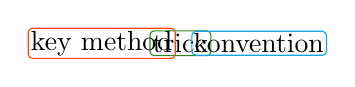
\begin{tikzpicture}
			\node [inner sep=1pt, rounded corners=1.5, draw=ForestGreen] (trick node) {trick};
			\node [inner sep=1pt, rounded corners=1.5, draw=OrangeRed, left of = trick node] {key method};
			\node [inner sep=1pt, rounded corners=1.5, draw=Cerulean, right of = trick node] (convention) {convention};
		\end{tikzpicture}
	}
	\blfootnote{\href{http://arxiv.org/abs/1607.02565}{(arXiv, 2016) DSO: Direct Sparse Odometry}}
	\blfootnote{\href{http://arxiv.org/abs/2312.06741}{(CVPR Highlight, 2024) MonoGS: Gaussian Splatting SLAM}}
\end{Frame}

\begin{Frame}{Keyframe Management: Prerequistes}
	\begin{enumerate}
		\setlength{\itemsep}{3ex}
		\item<+-> \alert<.>{What} is keyframing?
			\vspace*{1.5ex}
			\begin{itemize}
				\setlength{\itemsep}{1.5ex}
				\item<+-> A strategy of selecting and utilizing a subset of frames.
			\end{itemize}
		\item<+-> \alert<.>{Why} do we need keyframing?
			\vspace*{1.5ex}
			\begin{itemize}
				\setlength{\itemsep}{1.5ex}
				\item<+-> A \alert<.>{trade-off} between efficiency and accuracy/robustness/...
					\vspace*{1.5ex}
					\visible<+->{\par \alert<.>{infeasible} to optimize jointly on all frames online.}
			\end{itemize}
		\item<+-> \alert<.>{How} should we select keyframes?
			\vspace*{1.5ex}
			\begin{itemize}
				\setlength{\itemsep}{1.5ex}
				\item<+-> \alert<.>{non-redundant} and observing the \alert<.>{same area}.
				\item<+-> spanning a \alert<.>{wide baseline} for better multi-view constraints.
			\end{itemize}
	\end{enumerate}
	\blfootnote{\href{http://arxiv.org/abs/2312.06741}{(CVPR Highlight, 2024) MonoGS: Gaussian Splatting SLAM}}
\end{Frame}

\begin{Frame}{Keyframe Management: Registration}
	\blfootnote{\href{http://arxiv.org/abs/2312.06741}{(CVPR Highlight, 2024) MonoGS: Gaussian Splatting SLAM}}
	\begin{overprint}[\textheight]
		\par If \alert<+>{any} of the following conditions \alert<.>{is true}...
		\vspace*{\fill}
		\begin{block}<+->{\alert<.>{Small Gaussian Covisibility}\hfill Condition \romannum{1}, Keyframe Registration}
			Gaussian covisibility between the current frame and the previous keyframe drops below a threshold.
			\begin{figure}[htbp]
				\centering
				\resetcolorseries[3]{marknode-color-series}
				\resetcolorseries[3]{annotation-color-series}
				\begin{onlyenv}<.>
					\begin{equation*}
						\frac{\vert\operatorname{v}\left(\mathcal{G}, \mathcal{F}_{i}\right) \cap \tikzmarknode{n0}{\colorbox{marknode-color-series!![0]}{\(\operatorname{v}\left(\mathcal{G}, \mathcal{F}_{j}\right)\)}} \vert}{\vert\operatorname{v}\left(\mathcal{G}, \tikzmarknode{n1}{\colorbox{marknode-color-series!![1]}{\(\mathcal{F}_{i}\)}}\right) \cup \operatorname{v}\left(\mathcal{G}, \tikzmarknode{n2}{\colorbox{marknode-color-series!![2]}{\(\mathcal{F}_{j}\)}}\right) \vert} < \tau_1
					\end{equation*}
					\begin{annotatedEquationEnv}
						\annotatedEquation{colorseries}{n0}{north}{0em}{1em}{south west}{annotation-color-series}{\(\subset \mathcal{G}\), \textbf{visible} Gaussians from frame \(j\)}{east}
						\annotatedEquation{colorseries}{n1}{south}{0em}{-0.5em}{north east}{annotation-color-series}{the previous keyframe}{west}
						\annotatedEquation{colorseries}{n2}{south}{0em}{-0.5em}{north west}{annotation-color-series}{the current frame}{east}
					\end{annotatedEquationEnv}
				\end{onlyenv}
				\begin{onlyenv}<+->
					\vspace*{-2em}
					\begin{equation}
						\frac{\vert\operatorname{v}\left(\mathcal{G}, \mathcal{F}_{i}\right) \cap \operatorname{v}\left(\mathcal{G}, \mathcal{F}_{j}\right) \vert}{\vert\operatorname{v}\left(\mathcal{G}, \mathcal{F}_{i}\right) \cup \operatorname{v}\left(\mathcal{G}, \mathcal{F}_{j}\right) \vert} < \tau_1
					\end{equation}
					\vspace*{-2em}
				\end{onlyenv}
			\end{figure}
		\end{block}
		\vspace*{\fill}
		\begin{block}<.->{\alert<.>{Large Relative Translation}\hfill Condition \romannum{2}, Keyframe Registration}
			Translation from the previous keyframe w.r.t. to the median depth reaches a threshold.
			\begin{figure}[htbp]
				\centering
				\resetcolorseries[3]{marknode-color-series}
				\resetcolorseries[3]{annotation-color-series}
				\vspace*{-2em}
				\begin{onlyenv}<.>
					\begin{equation*}
						\frac{\Vert \mathbf{t}_{\mathcal{F}_i \mathcal{F}_j} \Vert_2}{\bar{D}_{\mathcal{F}_i \mathcal{F}_j}} > \tau_2, \quad \bar{D}_{\mathcal{F}_i \mathcal{F}_j} = \frac{1}{2 \tikzmarknode{n1}{\colorbox{marknode-color-series!![1]}{\(H\)}} \tikzmarknode{n2}{\colorbox{marknode-color-series!![2]}{\(W\)}}} \sum^{\{\mathcal{F}_i,\mathcal{F}_j\}} \sum_{h=0}^{H} \sum_{w=0}^{W} \tikzmarknode{n0}{\colorbox{marknode-color-series!![0]}{\(d(h,w)\)}}
					\end{equation*}
					\begin{annotatedEquationEnv}
						\annotatedEquation{colorseries}{n0}{south}{0}{-0.5em}{north west}{annotation-color-series}{depth of pixel \((h,w)\)}{east}
						\annotatedEquation{colorseries}{n1}{south}{0}{-0.5em}{north east}{annotation-color-series}{image height}{west}
						\annotatedEquation{colorseries}{n2}{south}{0}{-0.5em}{north west}{annotation-color-series}{image width}{east}
					\end{annotatedEquationEnv}
				\end{onlyenv}
				\begin{onlyenv}<+->
					\begin{equation}
						\frac{\Vert \mathbf{t}_{\mathcal{F}_i \mathcal{F}_j} \Vert_2}{\bar{D}_{\mathcal{F}_i \mathcal{F}_j}} > \tau_2, \quad \bar{D}_{\mathcal{F}_i \mathcal{F}_j} = \frac{1}{2 H W} \sum^{\{\mathcal{F}_i,\mathcal{F}_j\}} \sum_{h=0}^{H} \sum_{w=0}^{W} d(h,w)
					\end{equation}
					\vspace*{-2em}
				\end{onlyenv}
			\end{figure}
		\end{block}
	\end{overprint}
\end{Frame}

\begin{Frame}{Keyframe Management: Removal}
	\blfootnote{\href{http://arxiv.org/abs/2312.06741}{(CVPR Highlight, 2024) MonoGS: Gaussian Splatting SLAM}}
	\begin{overprint}[\textheight]
		\par If \alert<+>{any} of the following conditions \alert<.>{is true}...
		\vspace*{\fill}
		\begin{block}{\alert<.>{Beyond Window Capacity}\hfill Condition \romannum{1}, Keyframe Removal}<+->
			Remove the earliest keyframe out of the sliding window if the capacity is exceeded.
			\begin{equation}
				\vert \mathcal{W} \vert < \tau_3
			\end{equation}
		\end{block}
		\vspace*{\fill}
		\begin{block}{\alert<.>{Low Gaussian Overlap Coefficient}\hfill Condition \romannum{2}, Keyframe Removal}<+->
			Remove the previous keyframe if the ``Gaussian overlap coefficient'' between the previous frame and the new keyframe drops below a threshold.
			\begin{equation}
				\frac{\vert \operatorname{v}\left(\mathcal{G}, \mathcal{F}_{i}\right) \cap \operatorname{v}\left(\mathcal{G}, \mathcal{F}_{j}\right) \vert}{\min \left(\vert\operatorname{v}\left(\mathcal{G}, \mathcal{F}_{i}\right) \vert, \vert\operatorname{v}\left(\mathcal{G}, \mathcal{F}_{j}\right) \vert\right)} < \tau_4
			\end{equation}
		\end{block}
	\end{overprint}
\end{Frame}

\begin{Frame}{Gaussian Management: Insertion}
	\begin{itemize}
		\setlength{\itemsep}{1.5ex}
		\item<+-> \alert<.>{Why} do we need ``Gaussian insertion''?
			\vspace*{1.5ex}
			\begin{itemize}
				\setlength{\itemsep}{1.5ex}
				\item<+-> \alert<.>{SLAM} is for robotic exploration.
			\end{itemize}
	\end{itemize}
	\vspace*{\fill}
	\begin{itemize}
		\setlength{\itemsep}{1.5ex}
		\item<+-> \alert<.>{When} do we need ``Gaussian insertion''?
	\end{itemize}
	\begin{block}{\alert<.>{Keyframing}\hfill Condition \romannum{1}, Gaussian Insertion}<+->
		\par Insertion is triggered for every new keyframe.
	\end{block}
	\blfootnote{\href{http://arxiv.org/abs/2312.06741}{(CVPR Highlight, 2024) MonoGS: Gaussian Splatting SLAM}}
\end{Frame}

\begin{Frame}{Gaussian Management: Initialization}
	\begin{itemize}
		\setlength{\itemsep}{1.5ex}
		\item<+-> \alert<.>{How} do we insert Gaussians?
			\vspace*{1.5ex}
			\begin{itemize}
				\setlength{\itemsep}{1.5ex}
				\item<+-> Gaussian insertion is Gaussian \alert<.>{initialization}.
			\end{itemize}
	\end{itemize}
	\vspace*{\fill}
	\begin{block}{\alert<.>{If Depth Available}\hfill Gaussian Initialization}<+->
		Back-project in a per-pixel, per-Gaussian approach.
	\end{block}
	\vspace*{\fill}
	\begin{block}{\alert<.>{If Depth Unavailable}\hfill Gaussian Initialization}<+->
		Leverage the rendered depth map.
		\vspace*{1.5ex}
		\begin{itemize}[<+->]
			\setlength{\itemsep}{1.5ex}
			\item \alert<.>{for pixels with depth:} use the rendered depth and assign a ``low'' covariance.
			\item \alert<.>{for pixels w/o depth:} use the median of rendered depth and assign a ``high'' covariance.
		\end{itemize}
	\end{block}
	\blfootnote{
		In practice, ``low'': \(\sf 0.2 \sigma \); ``high'': \(0.5 \sigma\), where \(\sigma\) is the standard deviation of the rendered depth map.
	}
	\blfootnote{\href{http://arxiv.org/abs/2312.06741}{(CVPR Highlight, 2024) MonoGS: Gaussian Splatting SLAM}}
\end{Frame}

\begin{Frame}{Gaussian Management: Pruning}
	\begin{itemize}
		\setlength{\itemsep}{1.5ex}
		\item<+-> \alert<.>{Why} do we need ``Gaussian Pruning'' \textbf{if depth unavailable}?
			\vspace*{1.5ex}
			\begin{itemize}
				\setlength{\itemsep}{1.5ex}
				\item<+-> Too many \alert<.>{incorrect/unstable} newly inserted Gaussians.
			\end{itemize}
	\end{itemize}
	\vspace*{\fill}
	\begin{block}{\alert<.>{Low Gaussian Opacity} \hfill Condition \romannum{1}, Gaussian Pruning}<+->
		The Gaussians with a ``low'' opacity are pruned.
	\end{block}
	\vspace*{\fill}
	\begin{block}{\alert<.>{Low Gaussian Covisibility} \hfill Condition \romannum{2}, Gaussian Pruning}<+->
		For ``just'' inserted Gaussians but unobserved by ``some other'' keyframes, are pruned out.
	\end{block}
	\blfootnote{If no pruning, although the majority of incorrect Gaussians vanish quickly in following optimization, there are some survivals.}
	\blfootnote{In practice, the opacity threshold is \(\sf 0.7\).}
	\blfootnote{In practice, the pruned Gaussians are inserted in the last 3 keyframes and unobserved by any other 3 keyframes in the sliding window.}
	\blfootnote{\href{http://arxiv.org/abs/2312.06741}{(CVPR Highlight, 2024) MonoGS: Gaussian Splatting SLAM}}
\end{Frame}

\begin{Frame}{Mapping: Overview}
	\begin{center}
		\resizebox{!}{0.25\textheight}{
			\begin{forest}
				for tree={my tree}
				[
				Mapping
					[
						Bundle Adjustment
							[
								Photometric RGB \& Depth Loss,convention
							]
							[
								Isotropic Regularization,key
							]
							[
								Random Recall,trick
							]
					]
				]
			\end{forest}
		}
	\end{center}
	\pause
	\vspace*{\fill}
	\begin{itemize}
		\setlength{\itemsep}{1.5ex}
		\item<+-> \alert<.>{Why} do we need mapping in \textbf{3DGS} SLAM?
			\vspace*{1.5ex}
			\begin{itemize}
				\setlength{\itemsep}{1.5ex}
				\item<+-> \alert<.>{Local Mapping}: Optimize newly inserted 3D Gaussians.
				\item<+-> \alert<.>{Global Mapping}: Reconstruct a 3D-coherent structure.
			\end{itemize}
	\end{itemize}
	\blfootnote{
		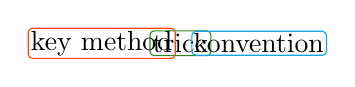
\begin{tikzpicture}
			\node [inner sep=1pt, rounded corners=1.5, draw=ForestGreen] (trick node) {trick};
			\node [inner sep=1pt, rounded corners=1.5, draw=OrangeRed, left of = trick node] {key method};
			\node [inner sep=1pt, rounded corners=1.5, draw=Cerulean, right of = trick node] (convention) {convention};
		\end{tikzpicture}
	}
	\blfootnote{\href{http://arxiv.org/abs/2312.06741}{(CVPR Highlight, 2024) MonoGS: Gaussian Splatting SLAM}}
\end{Frame}

\begin{Frame}{Mapping: Bundle Adjustment \& Random Recall}
	\begin{block}<+->{\alert<.>{Bundle Adjustment}}
		\begin{figure}[htbp]
			\centering
			\resetcolorseries[1]{marknode-color-series}
			\resetcolorseries[1]{annotation-color-series}
			\begin{equation}
				\underset{\mathcal{G}, \{\mathbf{T}_{cw}({\mathcal{F}_k})\vert \mathcal{F}_k\in \mathcal{W}\}}{\operatorname{argmin}} \sum_{\mathcal{F}_k}^{\tikzmarknode{n0}{\colorbox{marknode-color-series!![0]}{\scriptsize\(\mathcal{W}\)}}} \mathcal{L}_{pho}\left({\mathcal{F}_k}\right)
			\end{equation}
			\begin{annotatedEquationEnv}
				\annotatedEquation{colorseries}{n0}{north}{0em}{+0.5em}{south west}{annotation-color-series}{keyframes in the sliding window}{east}
			\end{annotatedEquationEnv}
		\end{figure}
		\vspace*{-1.5ex}
	\end{block}
	\vspace*{\fill}
	\begin{block}<+->{\alert<.>{Random Recall} \hfill A trick for global mapping}
		\vspace*{0.5ex}
		\par Besides \(\mathcal{W}\), ``some'' randomly selected past keyframes are also leveraged in BA to avoid forgetting the global map.
	\end{block}
	\blfootnote{\href{http://arxiv.org/abs/2312.06741}{(CVPR Highlight, 2024) MonoGS: Gaussian Splatting SLAM}}
\end{Frame}

\begin{Frame}{Mapping: Isotropic Regularization}
	\begin{itemize}
		\setlength{\itemsep}{1.5ex}
		\item<+-> \alert<.>{Why} do we need ``isotropic regularization''?
			\vspace*{1.5ex}
			\begin{itemize}
				\setlength{\itemsep}{1.5ex}
				\item<+-> \alert<.>{Observation:} isotropic Gaussians behave better than anisotrophic.
				\item<+-> \alert<.>{Analysis:} no constraints on the elongation along the viewing ray direction, \textbf{even with depth}.
			\end{itemize}
	\end{itemize}
	\vspace*{\fill}
	\begin{block}{Isotropic Regularization}
		\vspace*{0.5ex}
		\begin{equation}
			\mathcal{L}_{iso} = \sum_{i=1}^{\vert \mathcal{G} \vert} \Vert \mathbf{s}_i - \bar{\mathbf{s}}_i \Vert_1, \quad\text{where } \bar{\mathbf{s}}_i = \frac{1}{3} \left( s_i^{x} + s_i^{y} + s_i^{z} \right).
		\end{equation}
	\end{block}
	\blfootnote{\href{http://arxiv.org/abs/2312.06741}{(CVPR Highlight, 2024) MonoGS: Gaussian Splatting SLAM}}
\end{Frame}

\begin{Frame}{Mapping: Conclusion}
	\begin{block}{The Overall Optimization for Mapping}
		\begin{equation}
			\underset{\mathcal{G}, \{\mathbf{T}_{cw}({\mathcal{F}_k})\vert \mathcal{F}_k\in \mathcal{W}^{+}\}}{\operatorname{argmin}} \sum_{\mathcal{F}_k}^{\mathcal{W}^{+}} \mathcal{L}_{pho}\left({\mathcal{F}_k}\right) + \lambda_{iso} \mathcal{L}_{iso}
		\end{equation}
	\end{block}
	\blfootnote{\href{http://arxiv.org/abs/2312.06741}{(CVPR Highlight, 2024) MonoGS: Gaussian Splatting SLAM}}
\end{Frame}
